\documentclass[amsmath,amssymb,nofootinbib,12pt,preprint]{revtex4}
\usepackage{setspace}
%\doublespacing
\usepackage{graphicx}% Include figure files
%\usepackage{natbib}
\usepackage{color}
\usepackage{subfigure}
\usepackage{lscape}
\usepackage{hyperref}

\newcommand{\expo}[1]{{\rm e} ^{\left[ #1 \right] } } %quick way of writing e^
\nocite{*}


\begin{document}



\title{Geographical Voting Patterns in Berlin: \\ a Brief Data Science Case-Study.  }
\author{Brendan Osberg}

\date{\today}

\begin{abstract}

Voting data sets are a convenient platform for data science: they are quantifiable, controlled, and they exhibit the right balance of noise and signal. In Germany, in particular, the compulsory `Wohnmeldungs' allow for very detailed information in each riding. Moreover, in Berlin (as well as at the national level), the historical East/West divide provides a prominent feature for binary classification.
The results shown in this report represent the results of playing with this data a bit, primarily as a pedagogical tool for data science methodology.


That an ideological divide remains  between districts from the East and West has long been known qualitatively, however I want to  quantify it more precisely here and demonstrate that integration has actually succeeded in some demographics.
I start by performing cluster analysis on the $N=$1,779 districts of the city according to their vote-distribution among the major parties; \emph{three} clusters are observed. 

Two of the clusters, as expected, were overwhelmingly dominated by points east and west of the former wall respectively. A third cluster, however, was distributed almost exactly according to the null distribution of overall districts \---indicating that the barrier no longer has ideological significance to voters there. Where are these districts? More to the point: where exactly have efforts at integration been particularly successful? 

It turns out that it is in these regions where the Green party derives much of its support. What is it that the Green party are doing particularly well, compared to other parties in appealing to moderate (or `integrated') voters from both sides of the former wall?

\end{abstract}

\maketitle

%\section{Introduction.}
%
%\begin{itemize}
%\item Discuss historical significance of the wall  \--other popular outlets have certainly pointed out that divisions in political ideology across this historic boundary remain. We want to quantify it more precisely.  One of our major points of emphasis is that the failure of integration is not universal. \emph{Some} regions of the city have integrated far better than others, and we want to delineate where those regions are
%\item Describe k-means clustering and our test for robustness. For different k-values, groupings are highly influenced by the random initial conditions, implying that the clustering is arbitrary. For $k=3$, however, the same clusters are reproduced every time, meaning that this is a `real' clustering phenomenon.
%\end{itemize}

\section{ Methodology:}

\begin{itemize}
\item  I took publicly available data from the  1779 voting districts in Berlin from the 2016 election; Votes carried out by mail showed the same trend but lower sample size, thus we focus on the ``Urnenwahlbezirk"s.

\item All parties that received less than 5\% of the total vote were eliminated from the analysis. This preserved the $D=$6 `major'  parties in the following order: SPD, CDU, Green, Linke, AfD, and FDP.
 % (social democratic/labour), CDU (moderate conservative), Green (environmental), Linke (hard leftist; comprised of a lot of former DDR supporters), AfD (nationalist right-wing extremist), FDP (libertarian).

\item Each district was then assigned a `position' in the $D$-dimensional vector space of popular support for the major parties, without any regard to its geographical location. The proximity of points in this space can then be considered a measure of ideological consistency (i.e. two districts that are `close' to one-another in this vector space had a similar voting distribution among the six parties, regardless of their geographical location.)

\item We use the subscript $m\in [1,N]$ to index the riding (where $N=$1779), and the superscript $i\in [1,D]$ to index the political party, and we define a vector $v^{i}_{m}$ characterizing the vote shares assigned to each party $i$ in bezirk $m$. Normalization implies that 

\begin{equation}
\sum\limits_{i}^{D}v^i_m =1
\end{equation}

for all $v_m$. Furthermore, we can define the ideological vector (along various party lines) separating riding $m$ and $n$, as well as the magnitude of the distance separating them, using the Euclidean norm \footnote{ One might also consider KL divergence as a measure of distance since the elements aren't independent. Anecdotal observation suggests this is unlikely to make a significant difference.) } 

\begin{align}
\vec u_{mn} &=& \vec {v_m} - \vec{v_n} \\
\left| u_{mn}\right| &=& \sqrt{  \sum\limits_{i}\left( v_m^i - v_n^i \right)^2 }.
\end{align}

It is these distances that we use to define how the various voting bezirks are positioned relative to one-another in this $D$-dimensional ideological space.

\end{itemize}

%=======================================================================

\subsection{What patterns emerge from this data?}
The first question we wish to address: is there an ideological division between the East and West Berlin ridings in this ideological space? By taking a scatter plot of the points in the vector space described above, Fig.~\ref{fig:OstWest_div}, and the dimensionality-reduced Fig.~\ref{fig:tsne_OW} illustrate rather clearly that there is. This conclusion is not novel; newspapers reported on it extensively, but we can quantify it more precisely.

\begin{figure}[h]%
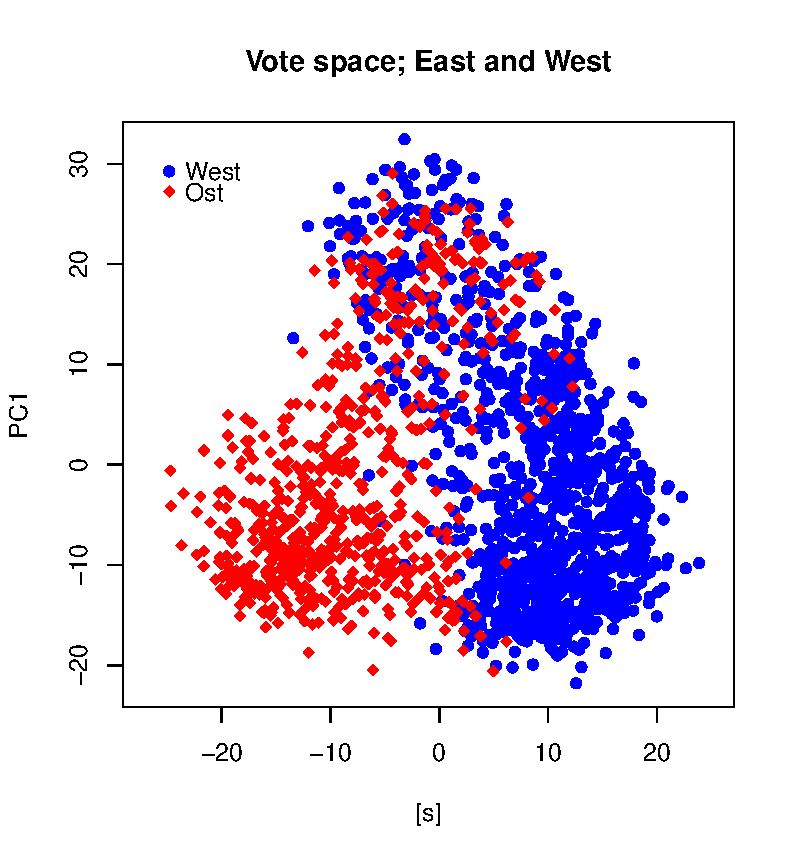
\includegraphics[scale=.85]{../figures/OstWest_Vote2}%
\caption{ Popular vote shares by district. Each point is one of the 1,779 districts, and the horizontal axis is defined by the average difference between East and West ridings. Blue points are West, red points are East, with location representing support among the major parties (the vertical axis is the first principle component among remaining axes). Units still correspond to percentage differences. }
\label{fig:OstWest_div}%
\end{figure}

\begin{itemize}
\item From Fig.~\ref{fig:OstWest_div}, it is clear that some division between eastern and western districts exist, and yet it is not clear whether data points near the top of the figure represent well-integrated districts, or whether there is some further separation along a dimension orthogonal to the plane. 


For this reason, the data are plotted again in a t-SNE plot in Fig.~\ref{fig:tsne_OW}, which reduces the set of full eight-dimensional distances between points into a two-dimensional separation.  The same data points from the top of the previous figure are shown well mixed in the bottom-right corner of Fig.~\ref{fig:tsne_OW}, indicating that there is, indeed a set of `well integrated' points.

\begin{figure}[h]%
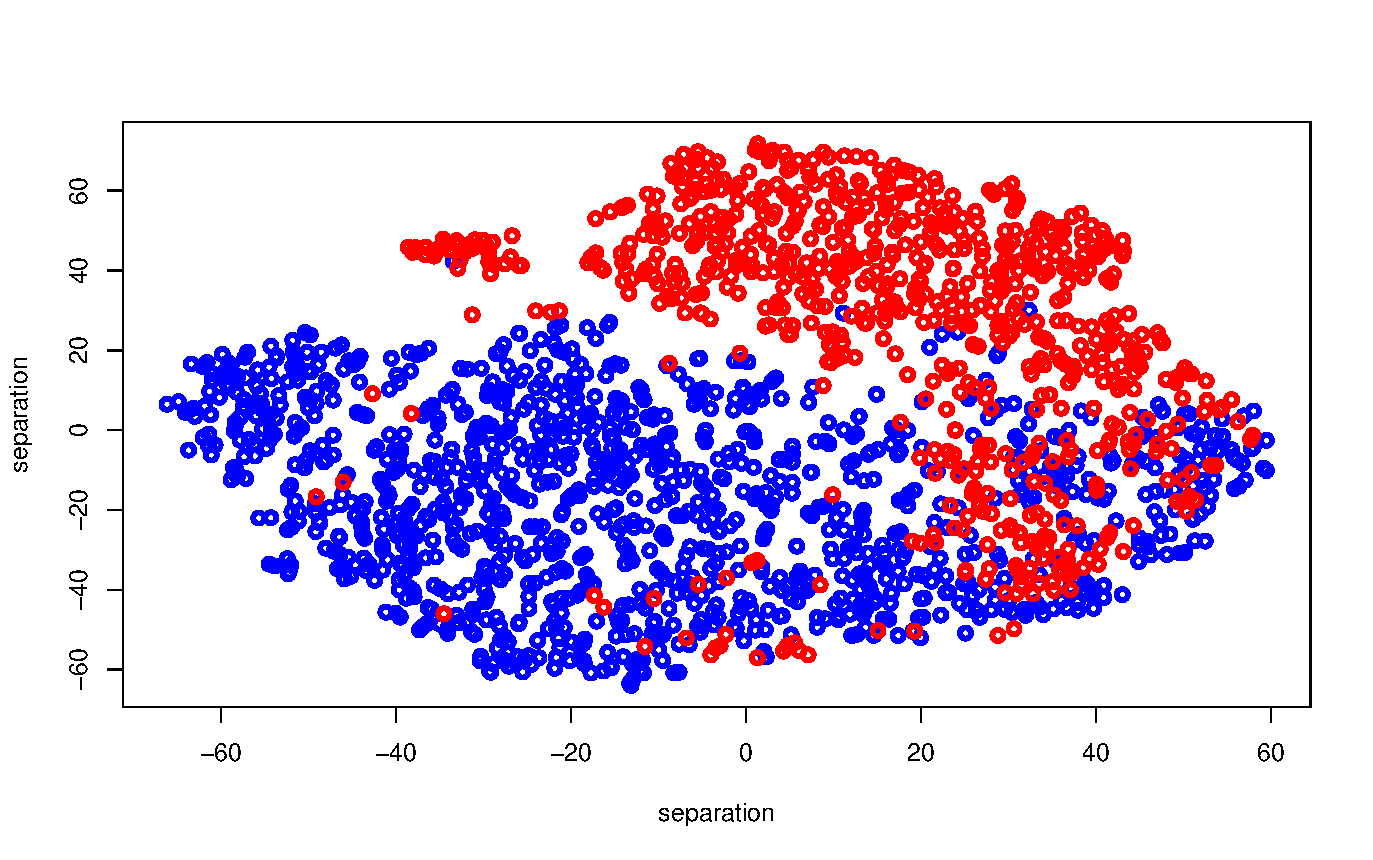
\includegraphics[scale=.5]{../figures/tsne_OstWest_Vote2}%
\caption{t-SNE plot of the same data from Fig.~\ref{fig:OstWest_div} color-coded red/blue for east/west. A t-SNE plot collapses the data into a two-dimensional figure where the lateral distance between each point $m$ and $n$ in the 2-D figure approximates $\left| \vec u_{nm}\right|$ the distance between the same two points in the full $D$-dimensional space.}
\label{fig:tsne_OW}%
\end{figure}

\subsection{clustering.}

\item To further emphasize this point, cluster analysis of these points was then performed using $k-$means clustering for various values of $k$. When $k$ was set to 2,4,5,6... it was observed that the clusters were not robust: stochastic initial conditions led to random assignment of the data points into each cluster\footnote{Here one might be interested in the Jacard index.}. With $k=3$, however, clusters were robust. In this case, we observed an `Eastern' cluster that was dominated by over 90\% ridings east of the wall; a `Western' cluster was, likewise, dominated by over 90\% ridings west of the wall. However, an `integrated' cluster was also observed, comprising of 65\% ridings from the West and 35\% ridings from the East, \---corresponding very closely to the null expectation of 60.4\% (Western) and 39.6\%(Eastern) districts overall.
\begin{figure}[t]%
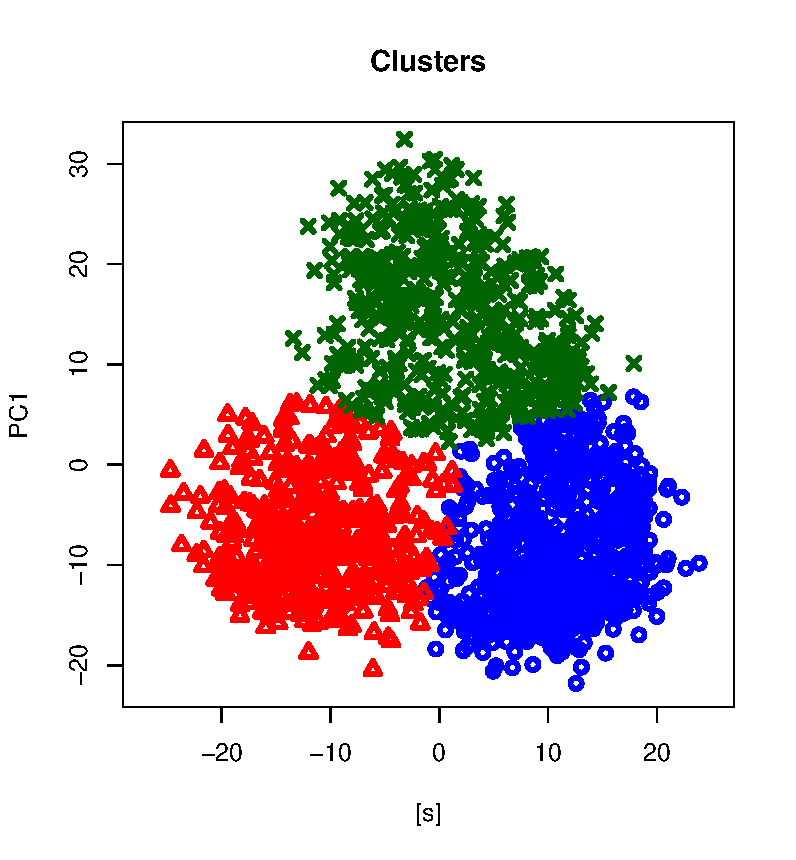
\includegraphics[scale=.85]{../figures/clusters_Vote2}%
\caption{The same data from Fig.~\ref{fig:OstWest_div} with data points color-coded by k-means clustering. When the `Integrated' cluster points are omitted, the separation between east and west dominated clusters increases to 25 percentage points. } 
\label{fig:clusters}%}
\end{figure}

\begin{figure}[h]%
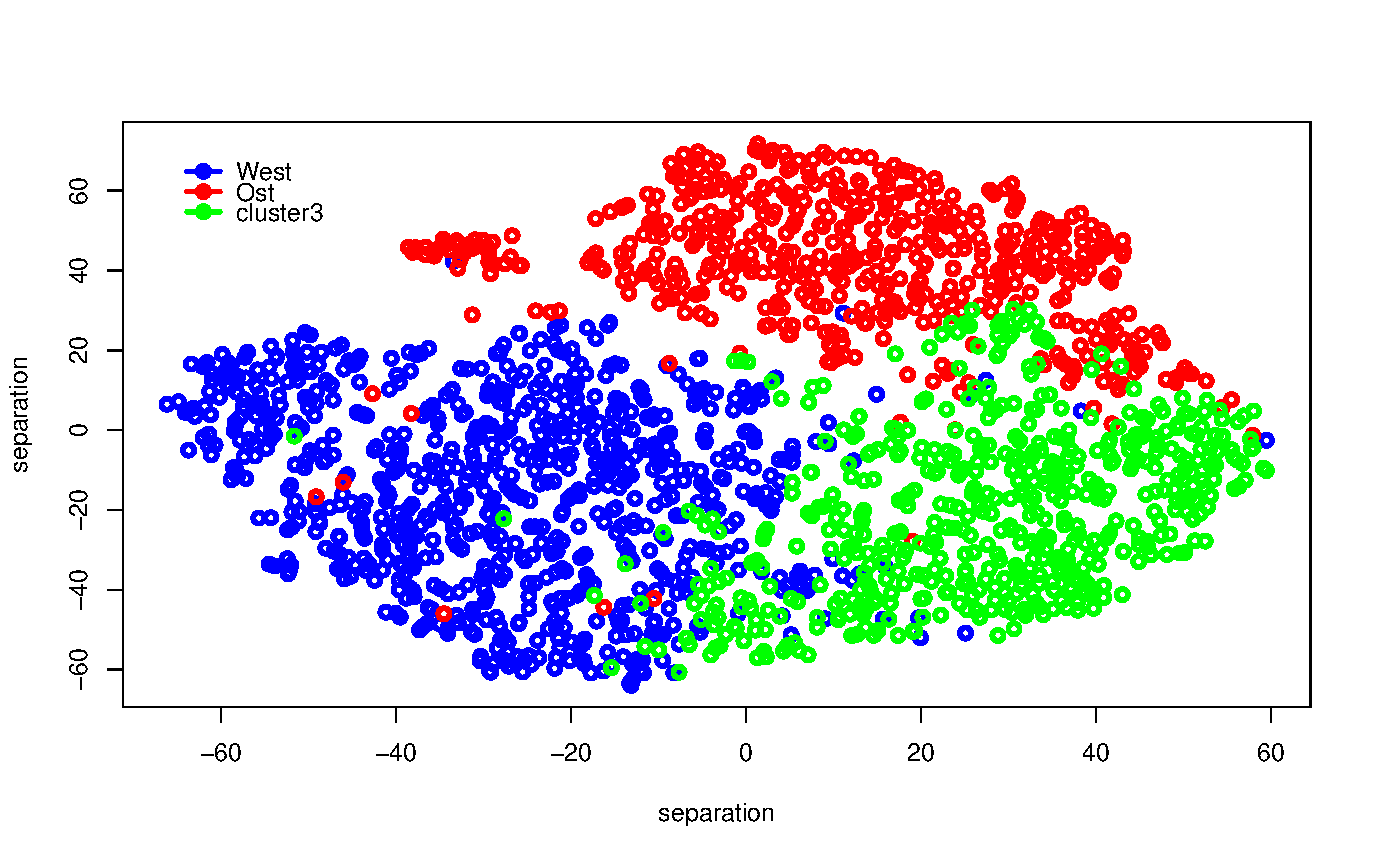
\includegraphics[scale=.5]{../figures/tsne_OW+C3}%
\caption{ The same data  as in \ref{fig:tsne_OW}, but with cluster 3 (the integrated region) color-coded green {\color{red} Note to self: do further color-coding to show the Eastern districts polarization into hard-left vs. hard-right }.}
\label{fig:tsne_C123}%
\end{figure}

\end{itemize}

Finally, Fig.~\ref{fig:barcluster} shows a bargraph of support for each major party by cluster. The SPD performs approximately equally well everywhere; The Eastern group tends to be polarized between East and West (based on high support for AfD and Die Linke), whereas the Western cluster is where the CDU performed particularly well. The Green party performed by far the best in the regions of the city where the East-West division was no longer significant.

\begin{figure}[h]%
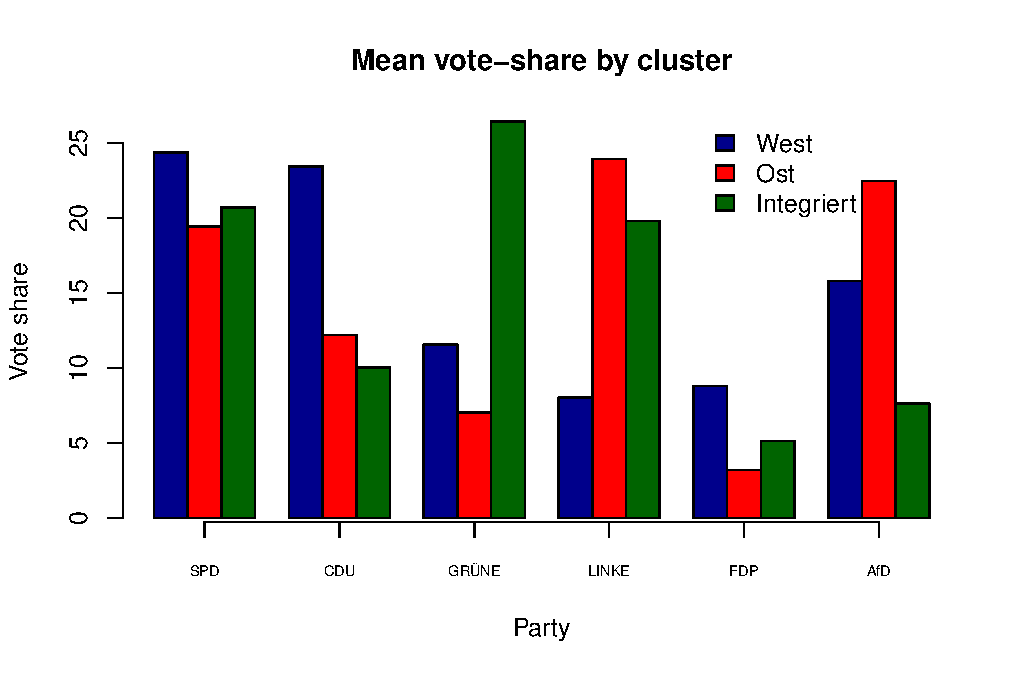
\includegraphics[scale=.75]{../figures/bargraph_vote2_6parties}%
\caption{Mean vote share among the major parties for each cluster.  } 
\label{fig:barcluster}%}
\end{figure}


\clearpage
\section{mapping successful integration}

So if we can see that there is a region where political integration is particularly successful, then where are these regions? Fig.~\ref{fig:map} shows the location of the above clusters on a map.
\begin{figure}[h]%
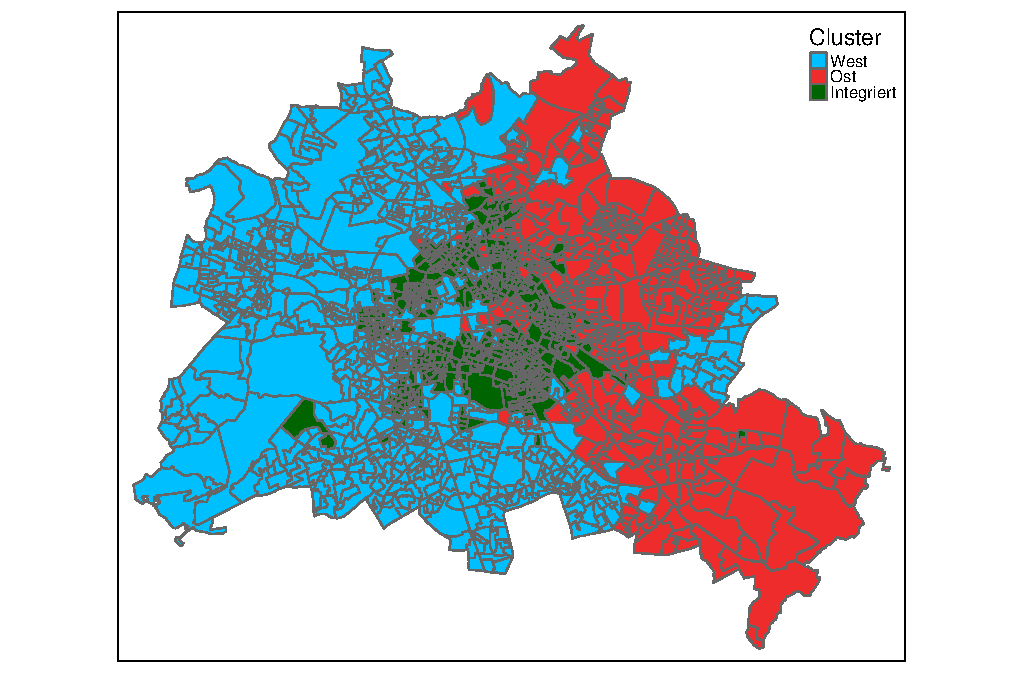
\includegraphics[scale=.85]{../figures/map_vote2_greenCC}%
\caption{ Map of Berlin with districts color-coded to indicate their cluster-assignment from Fig.~\ref{fig:clusters}. } 
\label{fig:map_vote2}%
\end{figure}

\begin{figure}[h]%
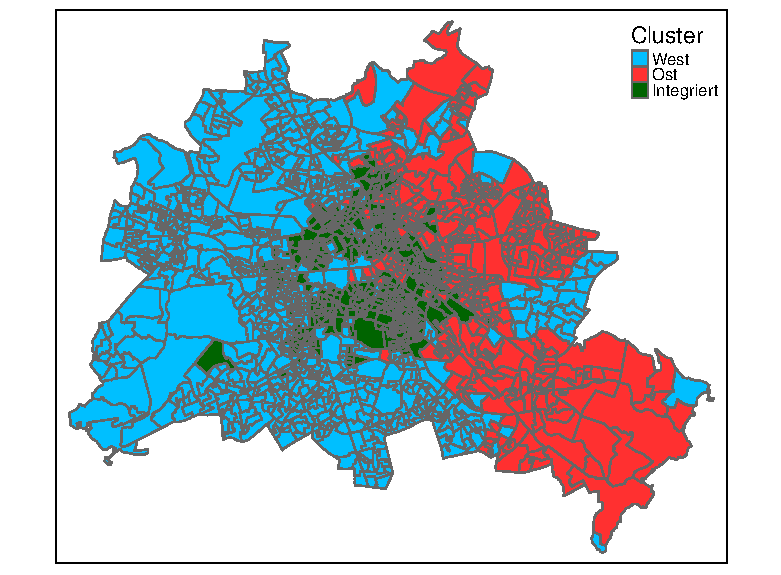
\includegraphics[scale=.85]{../figures/map_othercolorscheme}%
\caption{ Same map but using the results from the 1rst vote (i.e. based on candidate) -the results are almost identical.}
\label{fig:map}%
\end{figure}


We then consider the question: does this pattern conform to any observable feature of the city? Fig.~\ref{fig:bahntrace} shows the same map overlayed with the subway plan. Does support for the Green party coincide with the ``Ring bahn" --perhaps their supports live near S-bahn stations and take public transit rather than drive cars? perhaps Green voters are younger, more interested in environmental issues, less invested in historical divisions, and more likely to be renting apartments near the inner city rather than owning homes in the surrounding neighbourhoods?

\begin{figure}[h]%
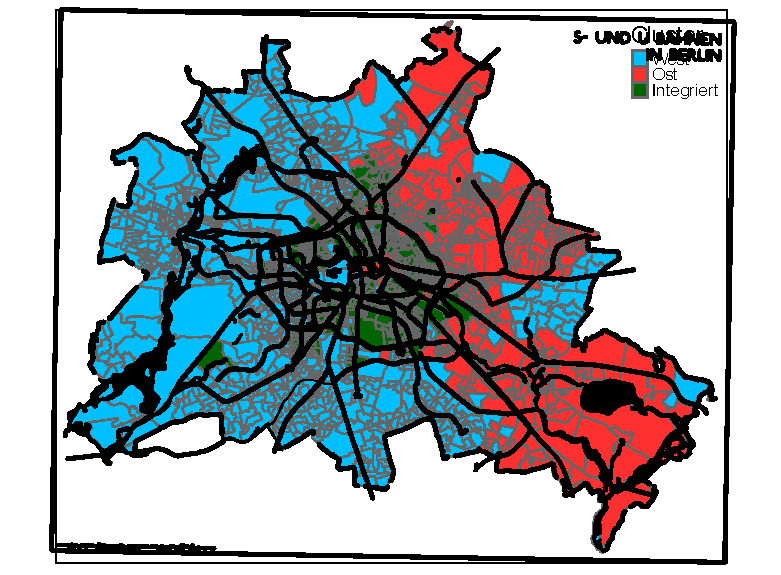
\includegraphics[scale=.85]{../figures/map_W_TRANSITTRACE}%
\caption{ The same data from Fig.~\ref{fig:map}, but with the U-bahn and S-bahn plan overlayed (unfortunately, the downloaded train lines that were obtained suffered from rendering issues in the resulting graph.) What other factors of the city might be correlated with this structure?}
\label{fig:bahntrace}%
\end{figure}

\clearpage

\section{What's actually causing this?}

We do not mean to imply that public transit is causing integration. Rather, this feature is symptomatic of a variety of other cultural and sociological factors: population density being one of the more obvious covariates. One might also consider, for example, the degree of immigration in a community (immigrants, presumably, being less attached to such a historical national division.) Fig.~\ref{fig:map_immigrant}, indeed, shows some correlation with this trend, in areas such as Neuk\"oln and Moabit, however, the above trend is apparently robust through the low-immigrant areas of PrenzlauerBerg and Wedding, while the latter appears alone in Charlottenberg.

\begin{figure}[h]%
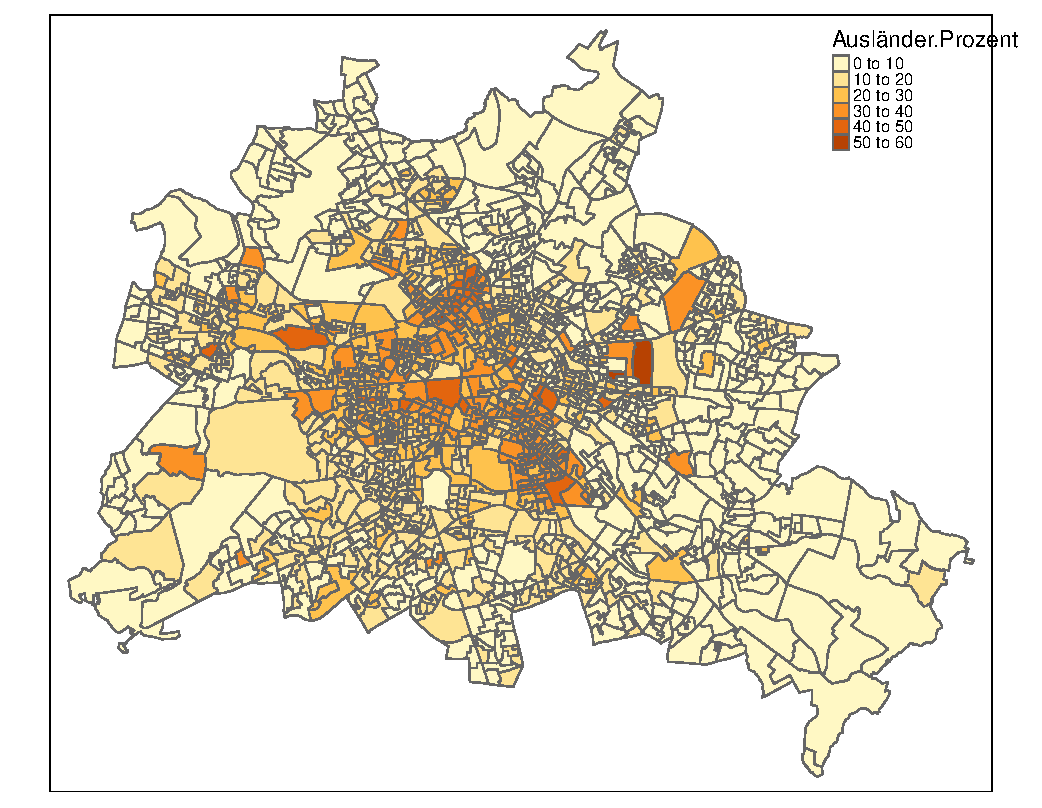
\includegraphics[scale=.65]{../figures/map_auslaender_prozent}%
\caption{ Percentage of the population immigrating from outside of Germany.}
\label{fig:map_immigrant}%
\end{figure}

We can also plot the age distributions: age ranges betwen 18-25, 45-60, and above 70 do not reveal much structure, however Fig.~\ref{fig:map_25-35} seems to show relatively high voter percentages among the age group 25-35, while Fig.~\ref{fig:map_60-70}, conversely, shows and anti-correlation among the age group 60-70.

\begin{figure}[h]%
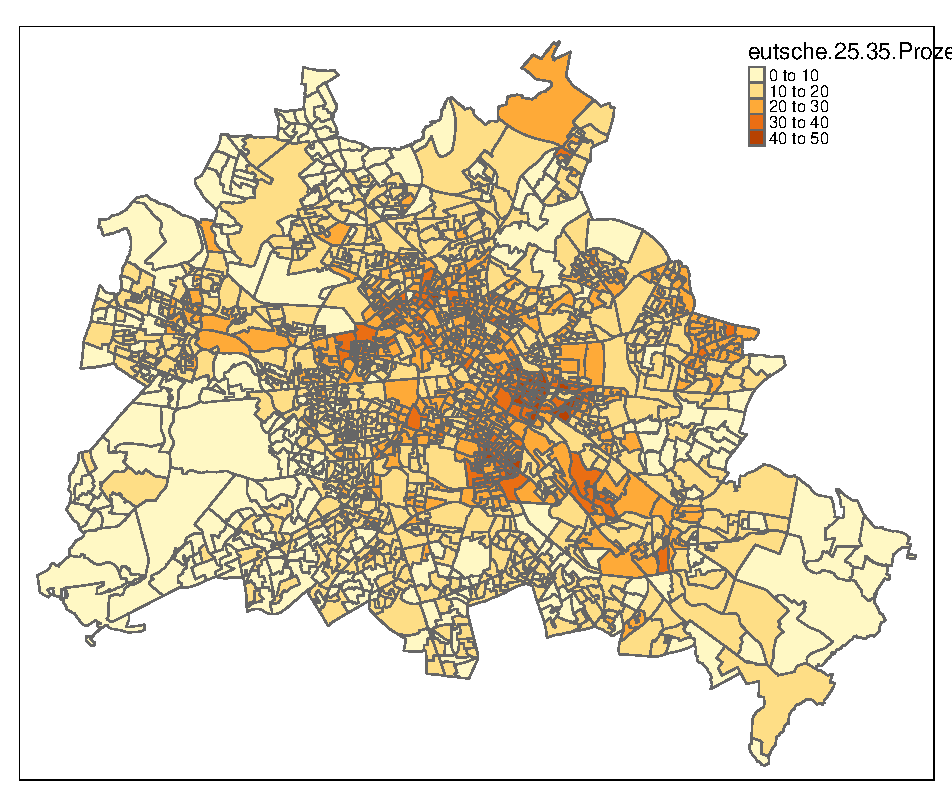
\includegraphics[scale=.65]{../figures/map_25-35}%
\caption{ Percentage of a ridings voters between the ages of 25 and 35: positive correlation with the Green `integrated' ridings is seen qualitatively {\color{red} calculate p-values and add them here}.}
\label{fig:map_25-35}%
\end{figure}

\begin{figure}[h]%
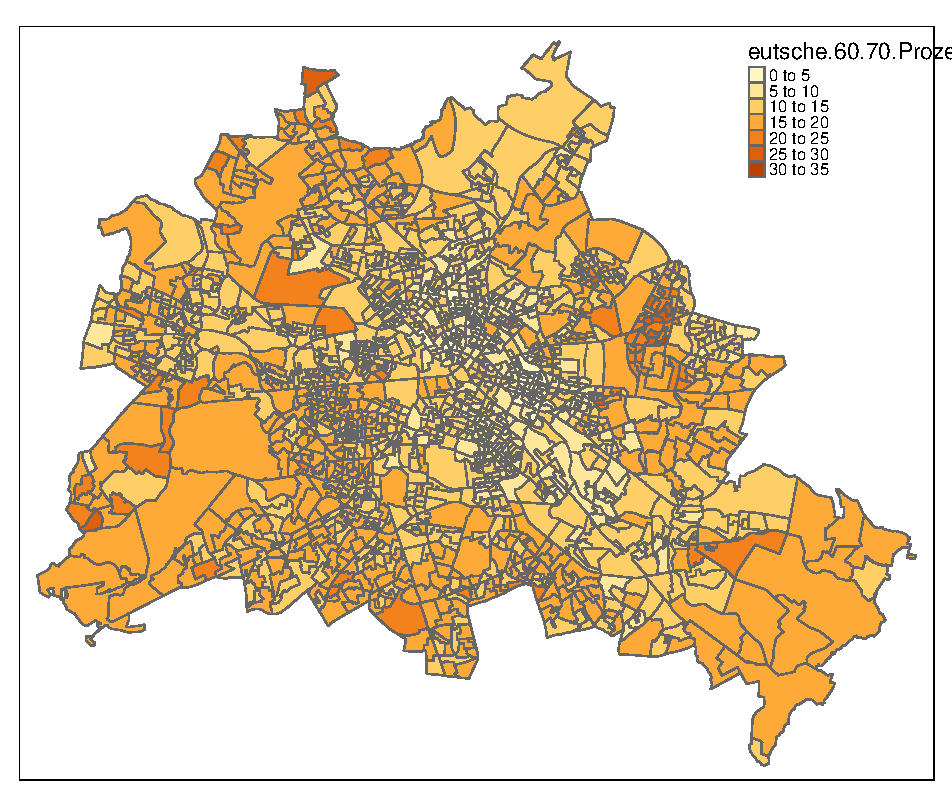
\includegraphics[scale=.65]{../figures/map_60-70}%
\caption{ Percentage of a ridings voters between the ages of 60 and 70: Anticorrelation with the Green-dominated integrated ridings is seen qualitatively, {\color{red} again: quantify this.}.}
\label{fig:map_60-70}%
\end{figure}

This would seem to paint a picture of integrated German society: Young and urbanized, but no strong correlation with immigration.

\clearpage

Other observations that can be made from this data: 
\begin{itemize}
\item The Eastern cluster tends to be more politically polarized, with both Die Linke and AfD drawing major support. On top of this, the sum of major party support among the West cluster was 99.2\%, while in the East cluster it was only 97.3\% meaning that in the East cluster, citizens were more than 3.5 times as likely to vote for Fringe parties (\emph{in addition} to their support for more radical parties such as AfD or die Linke) \footnote{It may be worthwhile to check the distribution of "invalid" votes, or people who abstained from voting at all \--perhaps this cluster correlates with turnout?.}
\item Look for outliers to the clustering trend:  e.g. that blue piece on the right that's physically east, but strongly ideologically `West', is that the same as the `tail' of red points at the bottom of Fig.~\ref{fig:OstWest_div}?
\item SPD support seems approximately uniform across the region \--why are they only party whose support is independent of region?

\item Why was Die Gr\"une so much higher in the integrated cluster?  Does concern for the environment seems to transcend historical divisions?
\end{itemize}


\section{What can be extended to the national level?}

I have not yet processed geo-data of the bezirks at the national level, though the same trends may well scale up at national level. However, the same cluster analysis can be done on previous years' national elections to look for the same trends; seeing how demographics have shifted since the last election might provide some predictive power to subsequent election.

I'd also like to extrapolate correlation on cluster support with turnout rates \--this would be particularly useful for party strategies: if the parties know what groups of people are supporting them, then they'd be interested to know where their efforts to get people to actually show up and vote are successful, and where they might need greater outreach. Before doing this, however, I thought it would be time-efficient to ask whether there is any interest in such results.

This, however, is a hobby project that I maintain occasionally alongside a full-time job. Hence, I have to be realistic about how much further time I can put in. If anyone would be interested in collaborating on this and sharing the work or taking it further and doing something more interesting with it please let me know and I'd be happy to hand over the code or run it for you (talk to me and I'm sure we can agree to some fair attribution).

\begin{thebibliography}{10}


\end{thebibliography}





\end{document}
